%プリアンブルは main.texの流用
%1. 基本設定
\documentclass[unicode, aspectratio=169, 12pt]{beamer}
%\usecolortheme[RGB={0, 139, 0}]{structure} %多分RGBで色を変えられる



% 2. 日本語設定（元々はこれだった，明朝体）
% fontspecは指定せず、標準の原ノ味フォント（TeX Live標準）に任せるのが最も安全です
%\usepackage{luatexja} 

% 2. 日本語設定（ゴシック体にフォント変更してみた）
% haranoajiを指定し、スライド全体の日本語デフォルトをゴシック体に変更する
\usepackage[haranoaji]{luatexja-preset}
\renewcommand{\kanjifamilydefault}{\gtdefault}
\renewcommand{\familydefault}{\sfdefault}




% 3. 数式・物理系のパッケージ
\usepackage{amsmath, amssymb, mathtools, bm}
\usepackage{physics} 
% physicsとの競合（\qty）を避ける設定で読み込みます
\usepackage[overwrite-functions=false]{siunitx} 
\usepackage{tensor} % テンソルをいい感じに描くためのパッケージ，それぞれのpcで使えるか要確認！！！！！！！！



% 4. 図・グラフ・枠組み（TikZ & tcolorbox）
\usepackage{graphicx}
\usepackage{tikz}
\usetikzlibrary{math, arrows.meta, angles, quotes, decorations.markings}
\usepackage[most]{tcolorbox} % 枠付きボックス（ascmacの代わりになります）



% 5. レイアウト設定
\renewcommand{\baselinestretch}{1.2} % スライドでは1.5は広すぎるため1.2程度が一般的です
\usepackage{url}

\newcommand{\diff}[2]{\frac{\mathrm{d} #1}{\mathrm{d} #2}} %常微分を書くパッケージ
\newcommand{\pdiff}[2]{\frac{\mathrm{\partial} #1}{\mathrm{\partial} #2}} %常微分を書くパッケージ

% 6. Beamerのデザインテーマ（Boadillaベース）
\usetheme{Boadilla}
\usecolortheme{whale}
\usefonttheme{professionalfonts}
\setbeamertemplate{navigation symbols}{} % 右下のアイコンを消す
\setbeamerfont{frametitle}{size=\Large, series=\bfseries}
\setbeamersize{text margin left=1cm, text margin right=1cm} %スライドの両端1cmを白紙にして寄りすぎないようにする
\setbeamertemplate{blocks}[rounded][shadow=false] %blockの下側の影を消す

% 7. タイトル情報
\title{オナーセミナー最終報告}
\author{笹伶夷\and 下橋以紗也\and 田處裕哉}
\institute{大阪大学 理学部 物理学科}
\date{\today}

\begin{document}

\begin{frame}{線の基本的な書き方}
    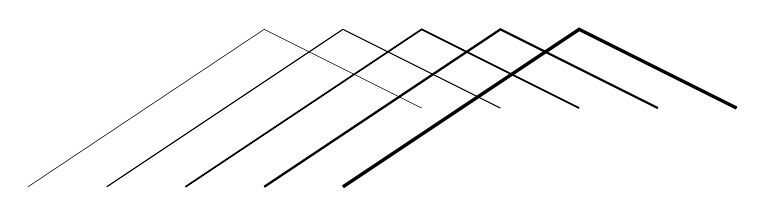
\begin{tikzpicture}[scale=1]
        %線の細さは　very thin, thin（これが標準）, semithick, thick, very thick, ultra thick
        \draw[very thin] (0,0)--(3,2)--(5,1);
        \draw[thin] (0+1,0)--(3+1,2)--(5+1,1);
        \draw[semithick] (0+2,0)--(3+2,2)--(5+2,1);
        \draw[thick] (0+3,0)--(3+3,2)--(5+3,1);
        \draw[very thick] (0+4,0)--(3+4,2)--(5+4,1);
    \end{tikzpicture}
\end{frame}

\begin{frame}{他の線の書き方(もっと太く，点線，矢印)}
    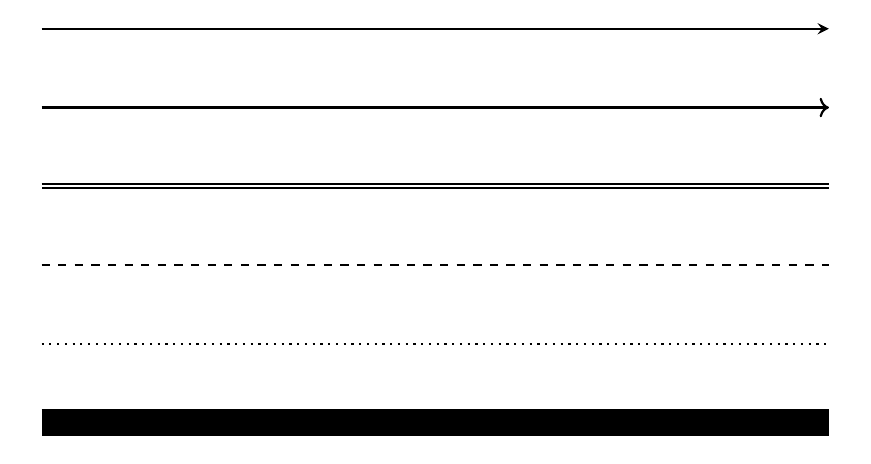
\begin{tikzpicture}
        %線のオプション
        \draw[line width = 10pt] (0,-1)--(10,-1);

        \draw[thick, dotted] (0,0)--(10,0); %点線
        \draw[thick, dashed] (0,1)--(10,1); %破線
        \draw[thick, double] (0,2)--(10,2); %二重線

        %矢印の書き方
        \draw[->,thick](0,3)--(10,3);
        \draw[->,> =stealth,thick](0,4)--(10,4);
    \end{tikzpicture}
\end{frame}

\begin{frame}{三角形を描いたり図中に文字を入れたり}
    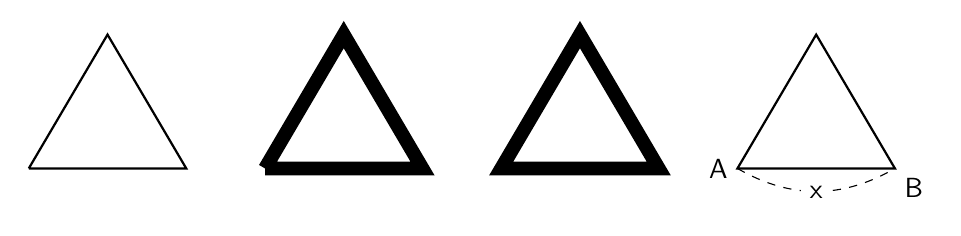
\begin{tikzpicture}

        \draw[thick](0,0)--(2,0)--(1,1.7)--(0,0);%三角形
        \draw[line width =5pt](0+3,0)--(2+3,0)--(1+3,1.7)--(0+3,0);%三角形を太くするとダサい
        \draw[line width =5pt](0+6,0)--(2+6,0)--(1+6,1.7)--cycle; %サイクルで書くとダサくない

        %文字の書き方
        \draw[thick](0+9,0)--(2+9,0)--(1+9,1.7)--cycle; 
        \draw(9,0)node[left]{A}; %\draw 座標 node[位置]{文字}で書く
        \draw(2+9,0)node[below right]{B}; %座標は above below left right の組み合わせで書くこともできる

        \draw[dashed](9,0)to[out =-30, in=210](11,0); %出発点と到着点に入る角度を度数法で指定すると曲線を書ける
        \draw(10,-0.3)node[fill = white]{x}; %node でfill=white をすると文字を書くためのスペースを作ることができる
    \end{tikzpicture}
\end{frame}

\begin{frame}{関数グラフを描く}
    \begin{tikzpicture}[scale=0.5]
        \draw[->,> =stealth, thick](-11,0)--(11,0)node[right]{x}; %x軸
        \draw[->,> = stealth, thick](0,-6)--(0,6)node[above]{y};  %y軸
        \draw(-10,0)node[below]{-10} (10,0)node[below]{10} (0,-5)node[right]{-5} (0,5)node[right]{5}; %見やすさのために座標を表示
        \draw(0,0)node[below left]{O}; %原点

        %とりあえず今はここまで，あとで続きもやる

    \end{tikzpicture}    
\end{frame}

\end{document}